%%%Template designed by Adam Glesser September 9, 2008
%%%All rights reserved (and deserved) 
%%%The only thing you should mess with on this line is the word problems.
%%%If this is a problem set, leave it as problems.
%%%If this is a solution set, change it to solutions.
\documentclass[12pt,solutions]{article}

%%%Here you should replace my name with your name
\newcommand{\prof}{Katie Henry \\ David Snyder \\ Adi Renduchintala}
%%%Make this your course number than leave it alone
\newcommand{\subj}{}
%%%Change the number 1 to which problem set you're on
\newcommand{\psnumber}{} %This is the Problem Set #
%%%Change the due date as needed
\newcommand{\duedate}{\date}  
%%%Change the topic as needed
\newcommand{\topic}{MLCD Project}


%%%%%%%%%%%%%%%You don't need to mess with anything in this section%%%%%%%%
\newif\ifisproblemset
\PassOptionsToClass{11pt,12pt}{article}
\DeclareOption{problems}{\isproblemsettrue}
\DeclareOption{solutions}{\isproblemsetfalse}
\ExecuteOptions{solutions}
\ProcessOptions\relax


\usepackage{amsmath, amssymb,bbold}
\usepackage{amsfonts}
\usepackage{multicol,parskip}
\usepackage{graphicx,booktabs}
\usepackage{tikz}
\usetikzlibrary{arrows,automata}
\usepackage{caption}
\usepackage{subcaption}
\usetikzlibrary{bayesnet}
\setlength{\oddsidemargin}{0pt} \setlength{\evensidemargin}{0pt}
\setlength{\textwidth}{6.5in} \setlength{\topmargin}{-.5in}
\setlength{\textheight}{8.5in}

\newlength{\toppush}
\setlength{\toppush}{2\headheight} \addtolength{\toppush}{\headsep}

%%%This command makes the title. Don't mess with it, unless you want to change the name Problem Set
%%%or Solution to Problem Set to something else.
\newcommand{\htitle} 
{
    \noindent\vspace*{-\toppush}\newline\parbox{6.5in}
    {
        \vspace{-.85cm}
        \prof\hfill \ 
	 \today
	\vspace*{-.5ex}\newline
        \mbox{}\hrulefill\mbox{}
    }
    \vspace*{1ex}\mbox{}\newline
    \begin{center}{
        \large\bf{A Method for Early Detection of Septic Shock Using Continuous Physiological Data
} }\end{center}
}

%%%This command makes the headers. Don't mess with it.
\newcommand{\handout}
{
    \thispagestyle{empty}
    \markboth{\topic}{\topic}
    \pagestyle{myheadings}
    \htitle
}



%%%%%%%%%%%%%%%%%%%%%%%%%%%%%%%%%%%%%%%%%%%%%%%%%%%%%%%%%%%%%%%%%%%%


%%%%%%%%%%%%This next section contains custom macros%%%%%%%%%%%%%%%%%%
%If these don't fit your course, remove them and add your own


%This first one allows you to write limits faster. It takes 4 inputs:
%The variable, what it's approaching, if relevant which side and the function.
%For example, if you wanted to write the limit as a x goes to 3 from the left 
%side of the function x^2 + 3, you would write $\limit{x}{3}{-}{x^2+3}$. If 
%you didn't care about which side you would leave the third set of braces empty, i.e.,
%$\limit{x}{3}{}{x^2+3}$.
\newcommand{\limit}[3]{\lim\limits_{#1 \rightarrow #2}\ #3}

  
%This is a slightly faster way of writing derivatives. It takes 2 inputs:
%The first is the function your differentiating, the second is the variable 
%with respect to which you're differentiating. For example, if you want to
%write the the derivative of y with respect to x, you would type $\d{y}{x}$.
\renewcommand{\d}[2]{\dfrac{\mathrm{d}#1}{\mathrm{d}#2}}  

%This last macro creates a multicolumn list environment where the first input is the number of columns.
%Use this command when you plan on having so many parts to a problem, with each being very short to state
%that you would like to put the problems in several columns. An example of the syntax would be 
%\multilist{3}{
%\item first item
%...
%\item last item
%}
%This will create a list that displays in 3 columns. The 3 can be replaced by any natural number, but 2 and 3
%are the only one numbers likely to give readable output.
\newcommand{\multilist}[2] 
    {
        \begin{multicols}{#1}
            \begin{enumerate}
                #2
            \end{enumerate}
        \end{multicols}
    }
%%%For solutions sets:
%%%After you write the problem, the next line should be
%%%\solution{Type your solution in here}
\newcommand{\solution}{ 
  \medskip
  {\bf Solution:}
}     

\newcommand{\argmax}{\operatornamewithlimits{argmax}}
\newcommand{\argmin}{\operatornamewithlimits{argmin}}
\newcommand{\half}{\frac{1}{2}}
\newcommand{\dx}{\frac{\delta}{\delta x}}
\newcommand{\ab}{\mathbf{a}}
\newcommand{\X}{\mathbf{X}}
\newcommand{\Y}{\mathbf{Y}}
\newcommand{\bA}{\mathbf{A}}
\newcommand{\bmu}{\boldsymbol{\mu}}
\newcommand{\x}{\mathbf{x}}
\newcommand{\Xs}{\tilde{\mathbf{X}}}
\newcommand{\xs}{\tilde{\mathbf{x}}}
\newcommand{\y}{\mathbf{y}}
\newcommand{\sx}{\bar{\x}}
\newcommand{\tb}{\mathbf{t}}
\newcommand{\SG}{\mathbf{\Sigma}}
\newcommand{\ts}{\theta^*}
\newcommand{\tbi}{t_{b_i}}
\newcommand{\ptb}{\hat{t}_b}
\newcommand{\tv}{t_v}
\newcommand{\tvi}{t_{v_i}}
\newcommand{\ptv}{\hat{t}_v}
\newcommand{\ps}{\hat{s}}
\newcommand{\yh}{\hat{y}}
\newcommand{\M}{\mathbf{M}}
\newcommand{\R}{\mathbb{R}}
\newcommand{\D}{\mathbb{D}}
\newcommand{\I}{\mathbb{I}}
\newcommand{\N}{\mathbb{N}}
\newcommand{\one}{\mathbb{1}}
\newcommand{\E}{\mathbb{E}}
\newcommand{\T}{\mathbf{T}}
\renewcommand{\S}{\mathcal{S}}
\renewcommand{\th}{t_0}
\newcommand{\w}{\mathbf{w}}
\newcommand{\W}{\mathbf{W}}
\newcommand{\p}{\mathbf{p}}
\newcommand{\wh}{\hat{\mathbf{w}}}
\newcommand{\wht}{\hat{\mathbf{w}}^T}
\newcommand{\whs}{\hat{\tilde{\mathbf{w}}}}
\newcommand{\whst}{\hat{\tilde{\mathbf{w}}}^T}
\newcommand{\ws}{\mathbf{w}^*}
\newcommand{\wst}{\mathbf{w}^{*T}}
\newcommand{\at}{\mathbf{a}^{T}}
\newcommand{\hth}{\hat{\theta}}
\newcommand{\bphi}{\boldsymbol{\phi}}
\newcommand{\btheta}{\boldsymbol{\theta}}
\newcommand{\dbphi}{\Delta\bphi}
\newcommand{\C}{\mathbf{C}}
\newcommand{\gd}{\nabla}
\newcommand{\hs}{\nabla^2}
\newcommand{\Cb}{\bar{C}}
\renewcommand{\labelenumi}{\arabic{enumi})}
\renewcommand{\labelenumii}{\alph{enumii})}
\providecommand{\norm}[1]{\lVert#1\rVert}

\newcommand{\solutionline}{
\begin{center}
\line(1,0){400}
\end{center}
}
    
%%%%%%%%%%%%%%%%%%%%%%%%%%%%%%%%%%%%%%%%%%%%%%%%%%%%%%%%%%%%%%%%%%%%%%%%%%%%%%%%%%%%
%%%%%%%%%%%%%%%%%%%%%%%%%%%%%%%%%%%%%%%%%%%%%%%%%%%%%%%%%%%%%%%%%%%%%%%%%%%%%%%%%%%%
%%%%%%%%%%%%%%%%%%%%%%%%%%%%%%%%%%%%%%%%%%%%%%%%%%%%%%%%%%%%%%%%%%%%%%%%%%%%%%%%%%%%
%%%%%%%%%%%%%%%%%%%%%%This is where the document begins%%%%%%%%%%%%%%%%%%%%%%%%%%%%%
%%%%%%%%%%%%%%%%%%%%%%%%%%%%%%%%%%%%%%%%%%%%%%%%%%%%%%%%%%%%%%%%%%%%%%%%%%%%%%%%%%%%
%%%%%%%%%%%%%%%%%%%%%%%%%%%%%%%%%%%%%%%%%%%%%%%%%%%%%%%%%%%%%%%%%%%%%%%%%%%%%%%%%%%%
%%%%%%%%%%%%%%%%%%%%%%%%%%%%%%%%%%%%%%%%%%%%%%%%%%%%%%%%%%%%%%%%%%%%%%%%%%%%%%%%%%%%
  
\begin{document}


%%%%%This stuff puts in the header and changes some spacing%%%%%%
\handout

\setlength{\parindent}{0pt}

The overall goal of this project is to develop a method for early detection of septic shock using continuous physiological data. We divide the problem into three parts: use HMM modeling to learn features from the physiological data, derive a decision policy to decide what if any state the system should predict, and use a neural network to estimate the conditional probabilities for each state.

%%%%%%%%%%%%%%%%%%%%%%%%%%%%%%%%%%%%%%%%%%%%%%%%%%%%%%%%%%
%%%%%%%%%%Here is where the actual math begins%%%%%%%%%%%%
%%%%%%%%%%%%%%%%%%%%%%%%%%%%%%%%%%%%%%%%%%%%%%%%%%%%%%%%%%
\setcounter{section}{0}
\section{Feature Discovery}
\subsection{Problem Definition}
The goal of this section is to detect hidden states over the time-series data for each patient, that would augment features being used by subsequent prediction systems. A natural model for such a system is the HMM. Using these hidden state sequences as input tokens of a document, we intend to run Topic models over all the patient records to see if there is any groups of states or any patten in state sequences that either explain or help predict the onset of septic shock.
\subsection{Related Works}
As noted in our proposal, the prognosis of septic shock in critically ill patients has a lot of variability. There is no single monolithic notion of septic shock \cite{Shavdia2007} . There are several methods to approach feature discovery in time series data of this nature. \cite{Esbroeck2012hrt}  applied symbolic aggregate approximation SAX \cite{Lin2003sax} on physiological time series data. More recently, Time series topic models have also been developed, \cite{SariaThesis2011} these work directly on continuous time domain signals and extract latent motifs. In our approach, we would like to investigate an HMM based approach, to allow a hidden state to emit a vector observation for a single time instance, where each element in the observation vector represents the observation of each channel of data (ECG, blood pressure, oxygen saturation etc).
\subsection{Contribution}
The dataset contains patient heart rate data at a frequency of 2 Hz. Each sample has been obtained by computing statistics over a 2 minute window from a the original heart rate data. Thus, every 120th sample represents statistics from a non-overlapping region from the original data. The first task is to extract these samples per patient record. We intend to find hidden states that best explain this lower resolution data. Each state of our HMM model will cover a wider time window, our current estimate for length of observation window per state is 10 minutes.\\
We also intend to extend the HMM to a coupled HMM where the second set of observations would represent blood pressure, temperature or oxygen saturation. Ideally the second set of observations would be in close time sync with the Heart rate data. This would be a factor in deciding which data stream (temperature, blood pressure or oxygen saturation) we would use for the second observation layer in the coupled HMM. Another factor would be the availability of these streams for all patient records. \\
\subsection{Learning Problem}
We propose to learn a HMM and then extend it to a coupled HMM. The 2 layers of observation are heart rate and blood pressure, temperature or oxygen saturation.  We intent to learn the states sequence that would best explain the patient records. Below is a representation of this coupled HMM, with each variable defined.\\
\begin{figure}[ht]
  \begin{center}
    \begin{tabular}{cc}
      % model_reclas

\begin{tikzpicture}

% define nodes

% decisions



\node[latent, minimum size=9mm] (z0) {$z_{t-1}$};
\node[latent, right=2 cm of z0, minimum size=9mm] (z1) {$z_{t}$};
\node[latent, right =2cm of z1, minimum size=9mm] (z2) {$z_{t+1}$};

\node[obs, above=2cm of z0, minimum size=9mm] (o3) {$o^2_{t-1}$};
\node[obs, right=2 cm of o3, minimum size=9mm] (o4) {$o^2_{t}$};
\node[obs, right =2cm of o4, minimum size=9mm] (o5) {$o^2_{t+1}$};

\node[latent, below=2cm of z0, minimum size=9mm] (y0) {$y_{t-1}$};
\node[latent, right=2 cm of y0, minimum size=9mm] (y1) {$y_{t}$};
\node[latent, right =2cm of y1, minimum size=9mm] (y2) {$y_{t+1}$};

\node[obs, below=2cm of y0, minimum size=9mm] (o0) {$o^1_{t-1}$};
\node[obs, right=2 cm of o0, minimum size=9mm] (o1) {$o^1_{t}$};
\node[obs, right =2cm of o1, minimum size=9mm] (o2) {$o^1_{t+1}$};





% edges

\edge {z0,y0} {z1};
\edge {z0,y0} {y1};
\edge {z1,y1} {z2};
\edge {z1,y1} {y2};

\edge {z0} {o3};
\edge {z1} {o4};
\edge {z2} {o5};

\edge {y0} {o0};
\edge {y1} {o1};
\edge {y2} {o2};

\end{tikzpicture}
    \end{tabular}
  \end{center}
  \caption{Coupled HMM model}
\label{fig:coupled_hmm_fig}
\end{figure}
\begin{align*}
O^1 &= o^1_{0}, \ldots,o^1_{T},   \text{sequence of heart rate observations (statistics from a 10 min time window)}\\
O^2 &=o^2_{0}, \ldots,o^2_{T},  \text{sequence of blood pressure or oxygen saturation}\\
Z &=  z_{0}, \ldots,z_{T}, \text{sequence of ${O^2}$ related states}\\
Y &=  y_{0}, \ldots,y_{T},  \text{sequence of ${O^1}$ related states}\\
\end{align*}
For this project deliverables, this model has been scaled down to a single HMM. Experiments were done to infer the feasibility of extracting useful information for prediction.\\
\subsubsection{State Priors}
The goal in this section is to provide an initial transition structure of the HMM model. The transition structure is can be depicted by figure 2.This automata shows that each patient starts from one of $n$ possible $Pre$ states. The $Pre$  states can be thought of as 'healthy' states before the $Onset$ of any of the 3 conditions that are being modeled. Of course there is no real 'healthy' state since all the records are from patients in the ICU. From each of the $Pre$ states the model can transition of any of the other $Pre$ states or it can transition to the $Onset$ state. This state, as the name suggests, is the onset of the condition being modeled. For a 'Sirs' patient , this state would signify the patterns in heart rate just before the a clinician can assign the label of 'Sirs' to the patient. This transition model suggests that once a patient is in the $Onset$ state they will continue to remain here until the $Post$ state. The $Post$ state can be thought of a the observations of patient heart heart just after they have been identified with one of the 3 conditions.
In the current model, a state can emit observations of a 10 minute window. Since the data has been down sampled to 1 sample per minute this results in each state benign a 10 dimensional mean vector, and a 10x10 dimensional covariance matrix.
\begin{figure}
\begin{center}
\begin{tikzpicture}[->,>=stealth',shorten >=1pt,auto,node distance=2.8cm,
                    semithick]
  \tikzstyle{every state}=[fill=white,draw=gray,text=black]

  \node[initial,state] (A)                    {$init$};
  \node[state]         (Pre2) [right of=A] {Pre1};
  \node[state]         (Pre1) [above of=Pre2] {Pre2};
  \node[state]         (Pre3) [below of=Pre2] {Pre3};
  \node[state]         (Onset) [right of=Pre2] {Onset};
  \node[state]         (Post) [right of=Onset]  {Post};

  

  \path (A) edge        node {$s$} (Pre1)
            edge              node {} (Pre2)
            edge              node  {}(Pre3)
        (Pre1) edge [loop above] node {$p$} (Pre1)
            edge  [bend left]node {$p$} (Pre2)
            edge  [bend left] node {$p$} (Pre3)
            edge  node {$o$} (Onset)
         (Pre2) edge [loop above] node  {}(Pre2)
            edge  node{} (Pre1)
            edge   node {} (Pre3)
            edge  node  {}(Onset)
         (Pre3) edge [loop below] node{}(Pre3)
            edge  [bend left]node  {}(Pre2)
            edge  [bend left] node{} (Pre1)
            edge  node{}  (Onset)
        (Onset) edge [loop above] node {$po$} (Onset)
        (Onset) edge  node {$po$} (Post)
        (Post) edge  [loop above] node {$e$} (Post);
\end{tikzpicture}
\end{center}
 \caption{Initial transition structure of HMM model}
\end{figure}
Using appropriate initial values for states is crucial to restrain the system from straying away from what might be explanatory data. We intend to encode some of our prior intuitions in this model in the following manner. Let ${Y}$ represent the states for heart rate observations over the patient record. We have the following insights from the data that we would like to encode.\\
1. Bootstrap from Patient Records: Each patient record has a time stamp representing the presence of SIRS, Sepsis, Severe Sepsis or Septic Shock. While this time stamps are not exact (that is, they are marked when the clinician happens to observe the symptoms and there is no guarantee that it was the precise moment of onset) we can still get statistics from the time region surrounding the clinicians observation of the symptoms. Using this technique we can get good initial guesses for statistics (such as means, and variances i.e. modeling the observation as a Guassian) for 4 states. It might also be preferable to model the observation given the state as a Beta distribution as we know that Heart rate can never be negative (which a gaussian in theory will allow).\\
2. Low Heart Rate Variability: Apart from the 4 states with we intend to bootstrap our model with states that have priors to restrict their parameters. One of the key insights regarding the onset of septic shock is reduction in heart rate variability. This informs us that one of the statistics that we need to compute from each 10 min time window should be a good indication of variability. Thus, simply getting mean heart rate for a 10 min duration would not be a good statistic. We intend to initialize a "Low Variability" state to capture this trend.
3. High Heart Rate Variability: The opposite state from the pervious would be the "High Variability" state where the 10 min window shows significant variation.\\
4. Reduction in Variability State: This state would be initialized such that there is variability across the earlier samples which slowly decline as we reach the end of the time window. One way to achieve this is to place a prior over the slope of a statistic such as change in variable from beginning of window to the end. A negative slope indicates reduction of variability.\\
\subsubsection{Model Training}
One way to capture all of these aspects is to initialize the mean and covariances of these states directly from the data. The $Pre$ states got their mean and variances from the first 10 min of data from each patient. The assumption here is that the beginning of a patient record is the time when they are relatively 'healthy' compared to the rest of their trajectory. In the figure above multiple $Pre$ states are shown, this is achieved by  perturbing the mean and setting it as the initial value for another state. This way the HMM can be modeled with an arbitrary number of states. The $Onset$ mean and covariance was obtained by computing the mean and covariance of 10 min windows just before the disease time stamp. The same was done to obtain the $Post$ state, except this represents the 10 min time window just after the disease label. We found that the initial states, actually did not appear to capture these trends. Since they were obtained by average across all patients with a particular disease condition, but after few iterations of EM over the model the mean values of the states seemed to show distinct forms.\\
%%%%%%%%
%% Show before after em states here
%%%%%%%%%

In the figure above (left) we see the means for 6 possible $Pre$ states for the Sirs condition. After 20 iterations of EM over the model we see the states each take on a specific characteristic(above right). 2 of the states represent high heart rate deviations, while 2 other represent low heart rate deviation. The most interesting states are those that capture the interesting changes in the heart rate. The Green line shows a 10 min window where the heart rate deviation is dropping and the purple line captures the opposite trend. With longer time windows it might be possible to capture more interesting patterns in this data.\\

Selection of number of states and selection of number of iterations are currently arbitrary. They both represent the extent to which the HMM models the training data. Increasing number of states and increasing the number of iterations could both lead to over fitting to the training data. To study to the performance of the model while keeping this is mind, a number of models each with different number of states and different number of iterations where trained. Thus each condition model (Sirs, Severe Sepsis and Septic Shock) 
the number of states ranged from 4 to 20, and the number of iterations from 2 to 100. 
\subsubsection{Evaluation}
Each trained state represents a characteristic trajectory over the window of observation.  Given a new observation sequence we can compute the best sequence of states that can be assigned to the observation sequence. This is also in a sense representing the original heart rate deviation as a series of interpretable states. But what is the predictive power of these model? After all any data will be fit by the EM algorithm as much as it can, and this will automatically result in a number of states. But how meaningful are these states in the context of prediction?\\
In an attempt to answer these questions, we tried to predict the instances of Septic Shock Vs Severe Sepsis Vs Sirs in the development data set. The assumption here is that each of these condition will have subtly different trajectories that can be detected before the onset stage. These subtle differences in trajectories should be captured by the Pre states of each model. Given a new unseen observation sequence, we can compute its forward probability under a model.  We choose the forward probability instead of the Viterbi probability because the Viterbi probability only represents the best state sequence, while forward probability is the sum of all possible state sequences a model can assign to the observation. A model that more closely fits the data would have higher forward probability.\\

A unseen development data set was created. Each condition model model that was trained was allowed to 'see' the initial observations of the unseen data. The range of initial observation were from 0-10 minutes, all the way to 0-1000 minutes in 20 minute increments. Using each initial observations a winning model was picked based on forward probability of the observation under that model. For example for patient 'A' the first 10 minutes of data was passed thought the Sirs, Severe Sepsis and Septic Shock models, if the Septic Shock model recorded that highest forward probability then its equivalent to predicting that patient 'A' is more likely to get Septic Shock. Clearly is more more the observation sequence is seen by each model, more reliable the forward probability estimates would be (in terms of relative likelihood). This trend is confirmed below by the plot of precision and recall of prediction of each model.

%%%%%%%%%%
%% insert precision recall plot here
%%%%%%
We can see that when small amounts of the observation is shown to each model (< 200 min) there is lot of fluctuation in the prediction. This makes sense because there is not enough data to get a reliable forward probability estimate. There is more chance of a model getting lucky since is just happened to have a state or two that matches closely with the small portion of data seen. We see that as the observations shown to the models increases there is more consistent prediction. Not only is the prediction more consistent, we also see fairly high precision and recall for 2 of the 3 conditions. The prediction of Septic Shock was made with a precision of ~0.7 and a recall of ~0.65, given that this is a three way prediction these represents accuracy substantially above chance. The figure was obtained by using models trained with 15 states and training was truanted at 100 iterations.\\

\subsubsection{Discussion}
We can also see that Severe Sepsis was never predicted. This results in very poor precision and recall for that class. This also makes sense because this condition is like a intermediate condition between Sirs and Septic Shock. This frame could not easily learn the subtle differences that separate Severe Sepsis from Sirs and Septic Shock.




\section{Neural Networks for Sepsis Prediction}

\subsection{Introduction}

\begin{figure}[h!]
  \caption{Schematic of a simple neural network}
  \centering
    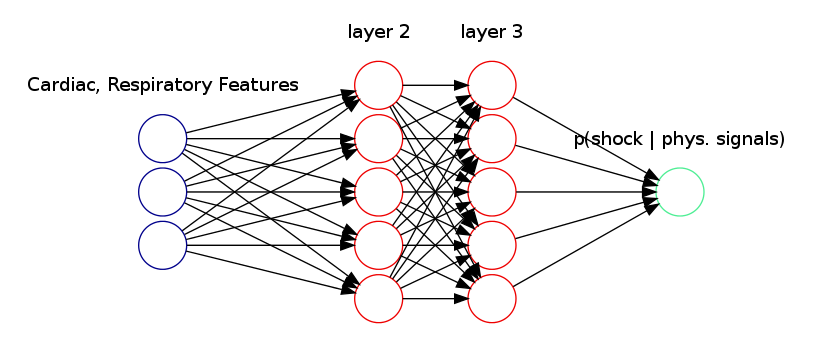
\includegraphics[width=1.0\textwidth]{nn_plots/nn}
\end{figure}

The goal of this section is to train neural networks to estimate the probability of developing a disease state given a sequence of
physiological data. Here, the task is early prediction of septic shock in ICU patients with a documented infection. Heart rate is used as input to the neural network. We estimate the probability of an ICU patient developing a form of sepsis $P(sepsis \mid S)$ where $S$ is a window of the 
heart rate timeseries. This model is motivated by the state of the art performance produced by Deep Neural Networks in a number of domains.


\subsection{Related Work}

The application of neural networks to the the task of sepsis prediction appears relatively unexplored. However, neural network techniques have been successfully applied to classification and prediction on other physiological time series. \cite{wulsin2011modeling} applied Deep Belief Networks (DBNs), a method related to Deep Neural Networks (DNN), to the task of anomaly detection in clinical EEG records. The group found that 
DBNs produced comparable results to other state of art methods, but significantly faster. They found
that using the raw EEG waveform showed improved performance in an
anomaly detection task over engineered features.
These results underscore the advantage of deep learning methods in 
automatically uncovering useful features. \\

To obtain adequate performance a body of techniques and tricks need to be considered. In \cite{hinton2012deep} speech recognition groups at Google, Microsoft, IBM and University of Toronto share various techniques for improving neural network performance. For instance, one should consider techniques for
preventing overfitting by certain restrictions on weight updating and smart initialization of weights.

\subsection{Approach}

Equation (\ref{eqn:sigmoid}) describes
the output of a neuron $j$ given the weighted commulative input $x_j$ (\ref{eqn:nn_x}). 
\begin{align}
y_{j} = \frac{1}{1+e^{-x_{j}}}
\label{eqn:sigmoid}
\end{align}
\begin{align}
x_{j} = b_{j} + \sum_{i}y_{i}w_{ij}
\label{eqn:nn_x}
\end{align}
\begin{align}
p(sepsis \mid S) = \frac{1}{1 + exp(x_{sepsis})}
\label{eqn:nn_prob}
\end{align}
\begin{align}
J = -\sum_{j} t_{j} log(y_{j})
\label{eqn:nn_J}
\end{align}
\begin{align}
\nabla J(w) = -\sum_{j} (y_{j} - t_{j}) x_{j}
\label{eqn:nn_dJ}
\end{align}
\begin{align}
input = \bar{x}_{1}, \sigma_{1}, \bar{x}_{2}, \sigma_{2}, ... ,\bar{x}_{60}, \sigma_{60}
\label{eqn:nn_input}
\end{align}

Equation (\ref{eqn:nn_prob}) represents the probability
of sepsis given some some sequence of physiological signals $S$. With only two classes, this is equivalent to the
\textit{softmax} function. The 
target function is (\ref{eqn:nn_J}) where $t_{j}$ is the correct class label (eg, sepsis or not sepsis). Equation (\ref{eqn:nn_dJ})
is the derivative at the output layer. Input to the network is a one hour frame in the form of a 2x60 vector of mean heart rate $\bar{x}$
and heart rate standard deviation $\sigma$. Each statistic is measured from a one minute interval in the original 2 Hz data.
\begin{align}
\eta = \frac{A}{\frac{epoch_{j}}{epoch_{max}} + 1}
\label{eqn:nn_eta}
\end{align}
\begin{align}
w_{i,j} \sim N(0, \frac{1}{\sqrt{inputs_{j}}})
\label{eqn:nn_w1}
\end{align}
\begin{align}
w_{i,j} \leftarrow \frac{w_{i,j}}{\sigma_{j}}
\label{eqn:nn_w2}
\end{align}
\\
Neural networks require careful weight initialization, pretraining (for deep networks), topology and other considerations 
described in \cite{vesely2013sequence, hinton2012deep}. To help guarantee convergence, we have a learning rate which decreases as the 
number of epochs increase (\ref{eqn:nn_eta}). Weights are drawn from a normal distribution (\ref{eqn:nn_w1}), which we found offered greater stability over alternative distributions, such as uniform. After two or three hidden layers, the network suffers from oversaturation, which is characterized by a very large range of values from the
transfer functions in (\ref{eqn:sigmoid}), resulting in numerical overflow and underflow. To combat this issue, we simply divide by the standard deviation
of the weights in the oversaturated layer during training (\ref{eqn:nn_w2}).
\\
We use a standard batch gradient descent backpropagation algorithm to train the network. We experimented with stochastic gradient descent and didn't
notice much of an advantage. Moreover, it's easier to track the training process in batch gradient descent: at each epoch, we calculate
the loss function (\ref{eqn:nn_J}) and in the batch variation, we can be sure that the network's parameters have been altered by every training example.

\subsection{Preliminary Results and Evaluation}

\begin{figure}
        \centering
        \begin{subfigure}[b]{0.4\textwidth}
                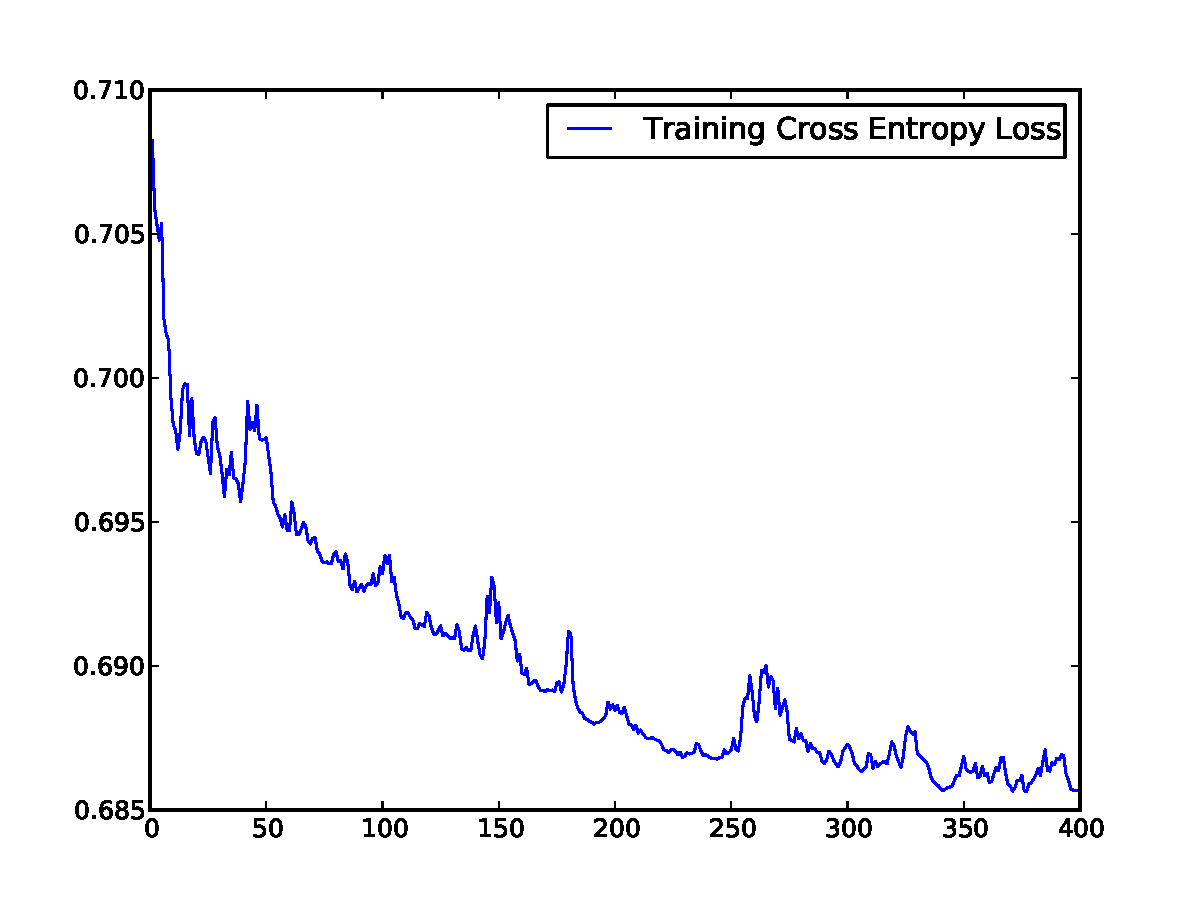
\includegraphics[width=\textwidth]{nn_plots/loss2}
                \caption{Cross entropy loss vs. number of epochs.}
                \label{fig:entropy}
        \end{subfigure}
        \begin{subfigure}[b]{0.4\textwidth}
                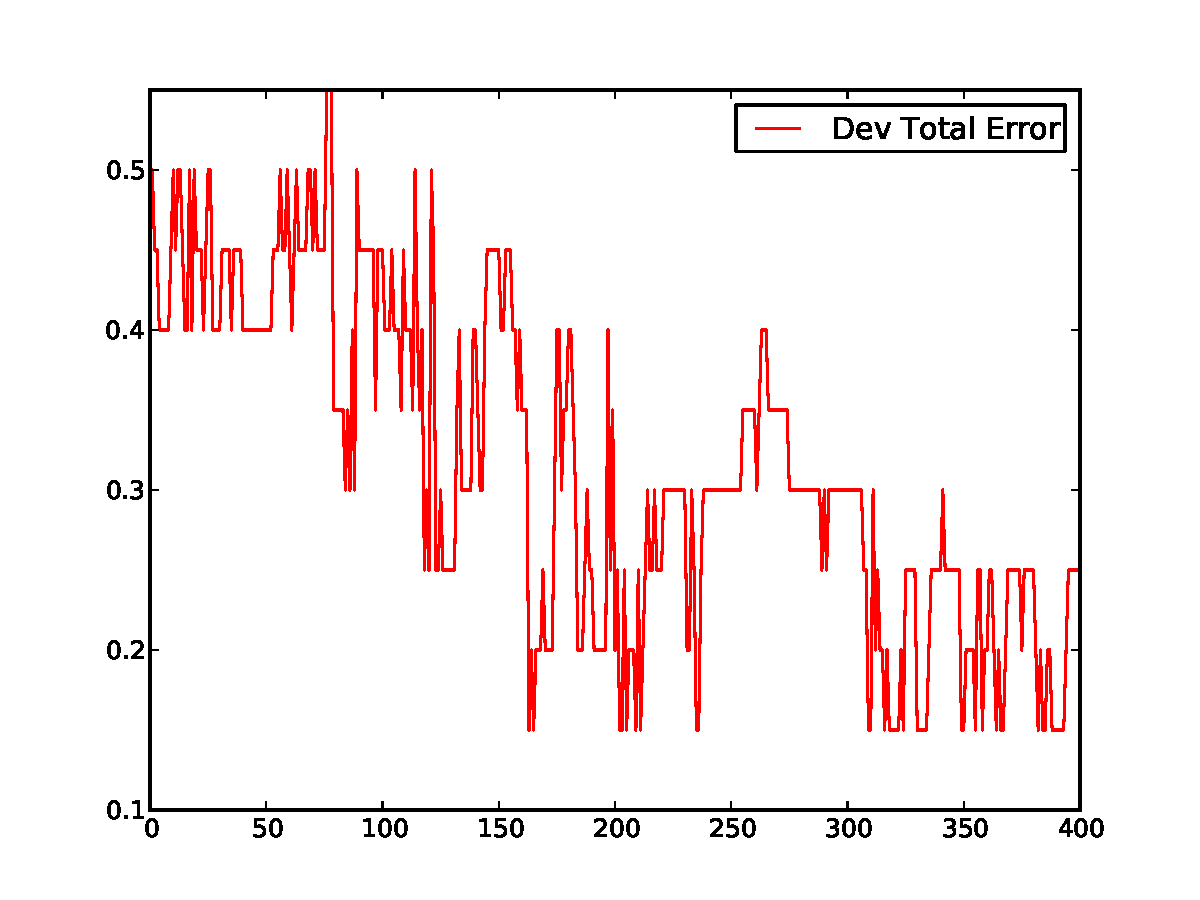
\includegraphics[width=\textwidth]{nn_plots/dev2}
                \caption{Development (validation) set error rate vs. number of epochs.}
                \label{fig:dev}
        \end{subfigure}
\caption{Typical results for a network with 120 input nodes, 1 hidden layer with 100 nodes, and one output layer with 1 node.}\label{fig:loss_dev}
\end{figure}

In figure \ref{fig:loss_dev} we present typical results for a network with 120 input nodes, 1 hidden layer with 100 nodes, and a single output layer with 1 node. Given the current framework, we didn't see an advantage in using more than 1 hidden layer. The development (validation) error rate
in ~\ref{fig:dev} is the classification error rate. To obtain classification from the conditional probabilities generated by the network, we
map probabilities at or above 0.5 to class 1, and probabilities below 0.5 to class 0.
\\
\\
To train the network in figure ~\ref{fig:loss_dev} we do not use a sliding window over the entire time series for each patient. Instead, we 
first separate the data into two categories: SIRS, and severe sepsis and septic shock. From the SIRS category we randomly select some
number of 1 hour frames. From the severe sepsis and septic shock category, we only select the one hour frames which immediately precede 
the onset of the disease. While this setup isn't ideal, it plays an important step in the goal of more sophisticated prediction, by
demonstrating that we can distinguish between certain disease states by using just heart rate.

\begin{figure}
        \centering
        \begin{subfigure}[b]{0.4\textwidth}
                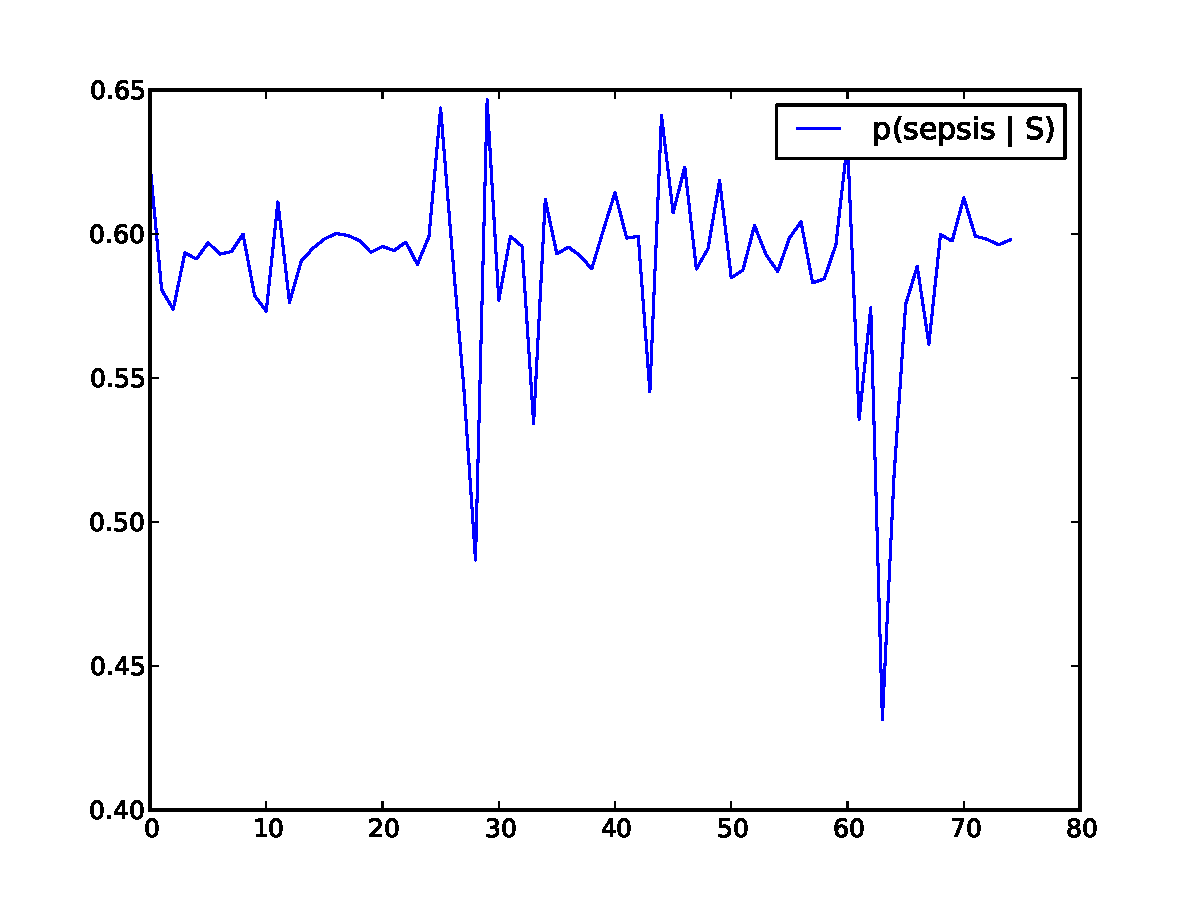
\includegraphics[width=\textwidth]{nn_plots/probs_c0_1}
                \caption{}
                \label{fig:c0_0}
        \end{subfigure}
        \begin{subfigure}[b]{0.4\textwidth}
                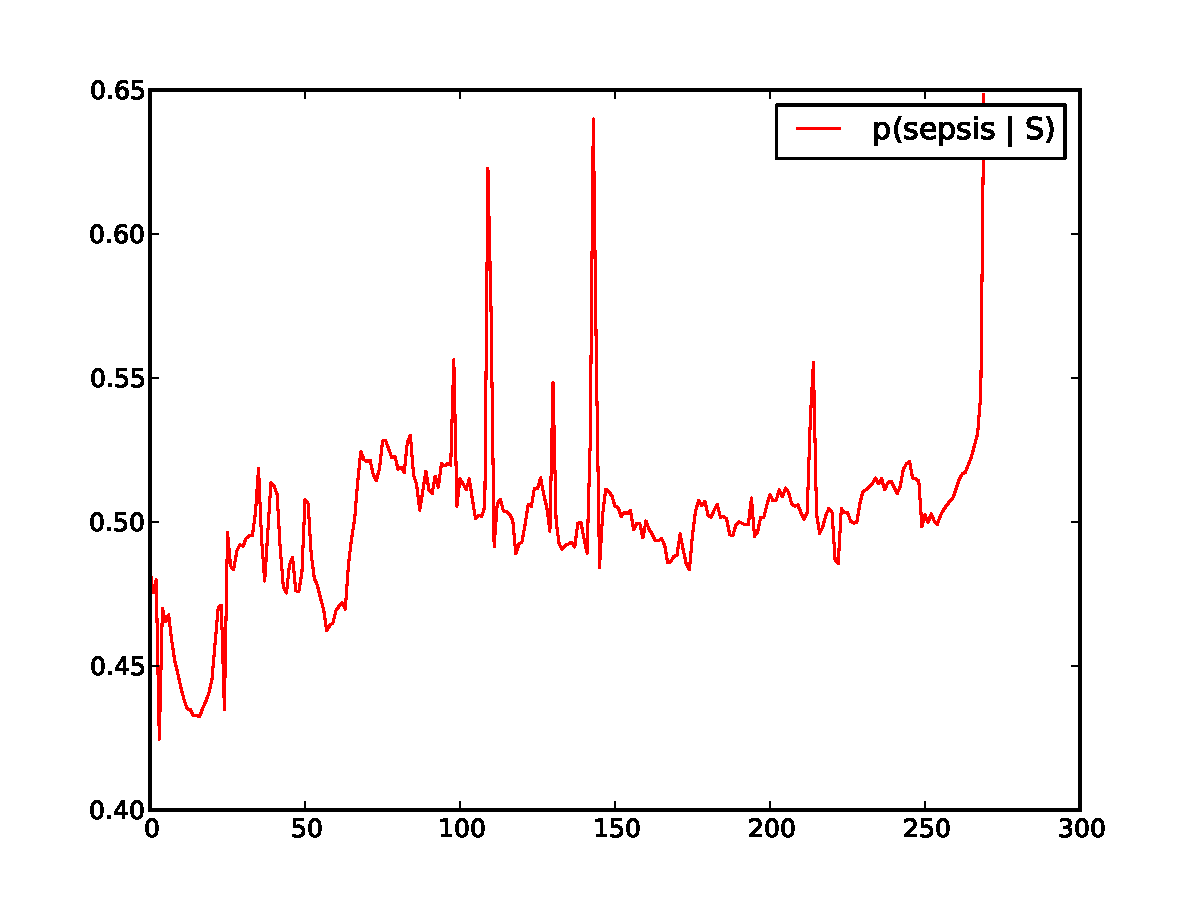
\includegraphics[width=\textwidth]{nn_plots/probs_c1_2}
                \caption{}
                \label{fig:c0_0}
        \end{subfigure}
        \begin{subfigure}[b]{0.4\textwidth}
                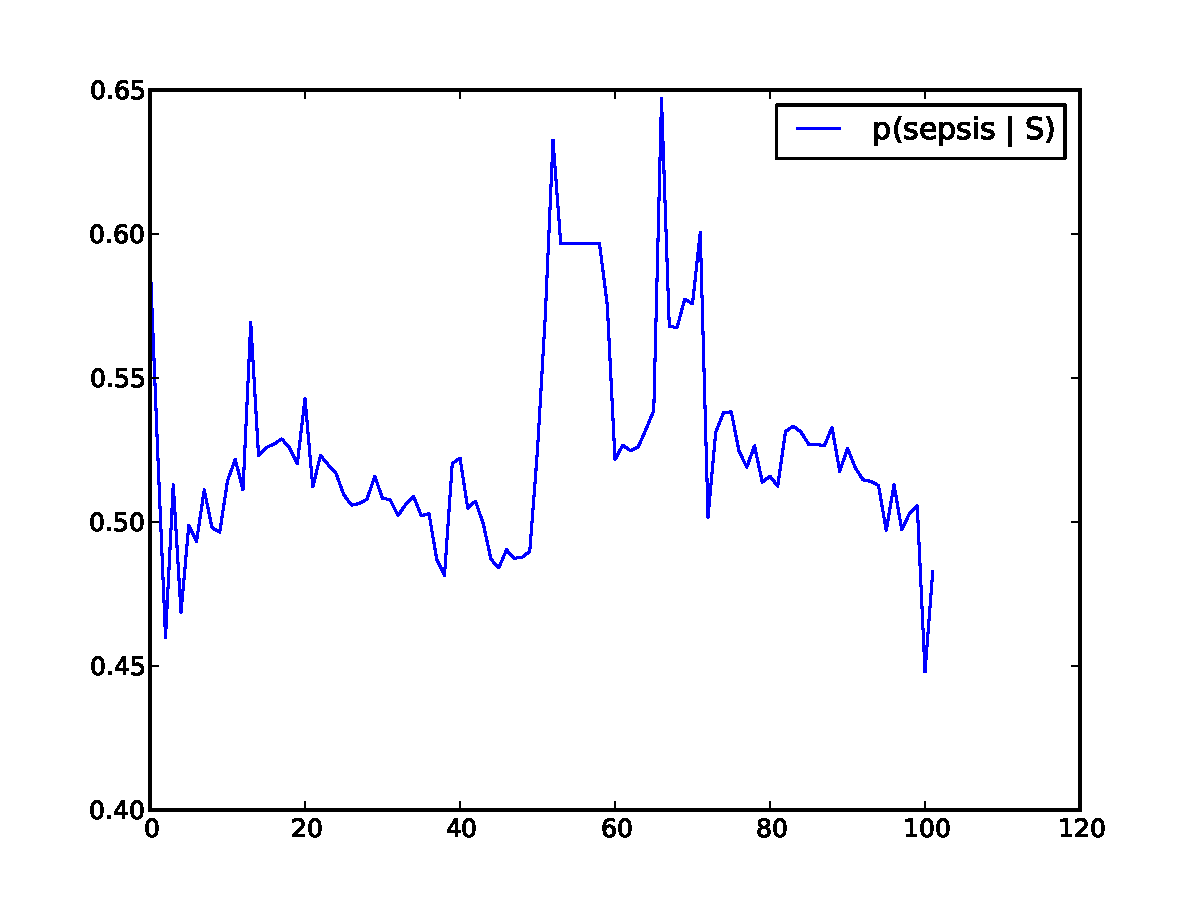
\includegraphics[width=\textwidth]{nn_plots/probs_c0_3}
                \caption{}
                \label{fig:c0_0}
        \end{subfigure}
        \begin{subfigure}[b]{0.4\textwidth}
                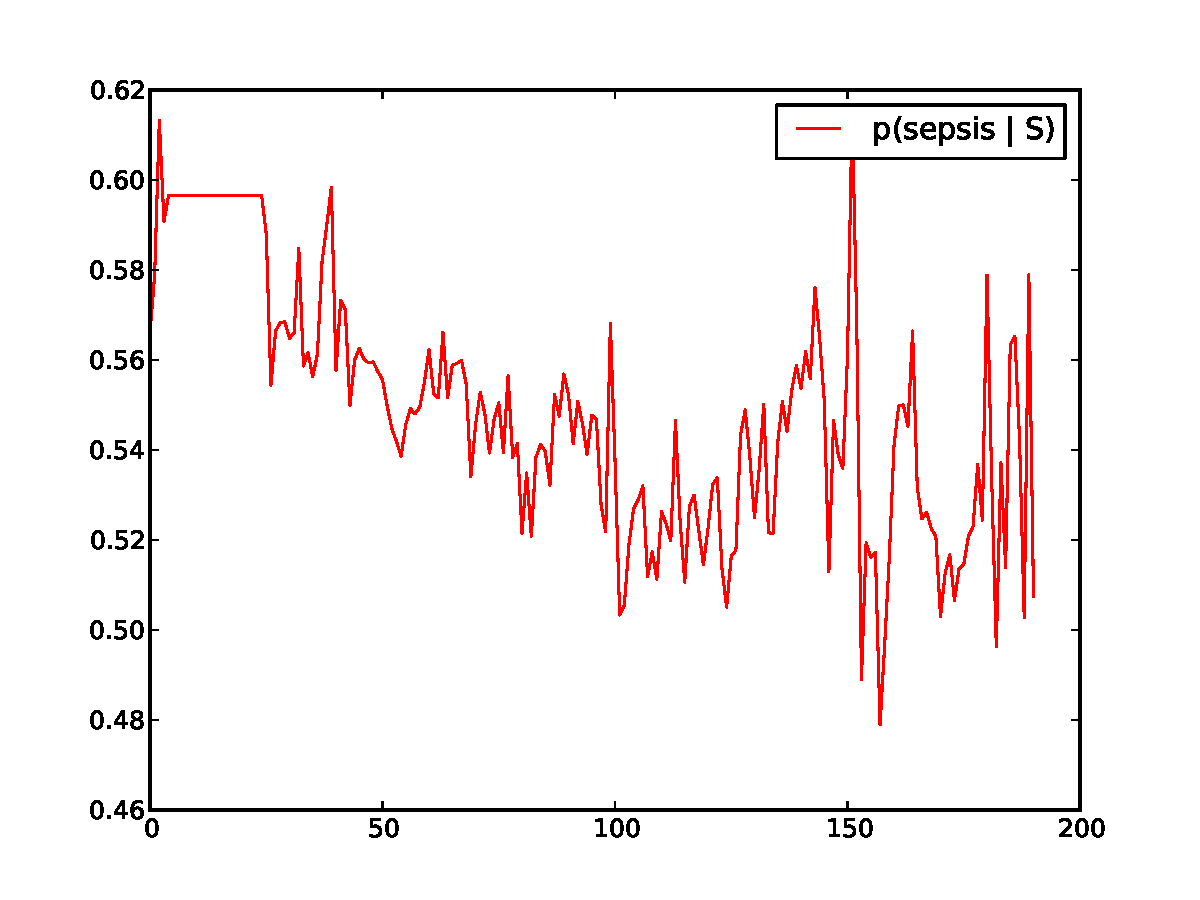
\includegraphics[width=\textwidth]{nn_plots/probs_c1_3}
                \caption{}
                \label{fig:c0_0}
        \end{subfigure}
        \begin{subfigure}[b]{0.4\textwidth}
                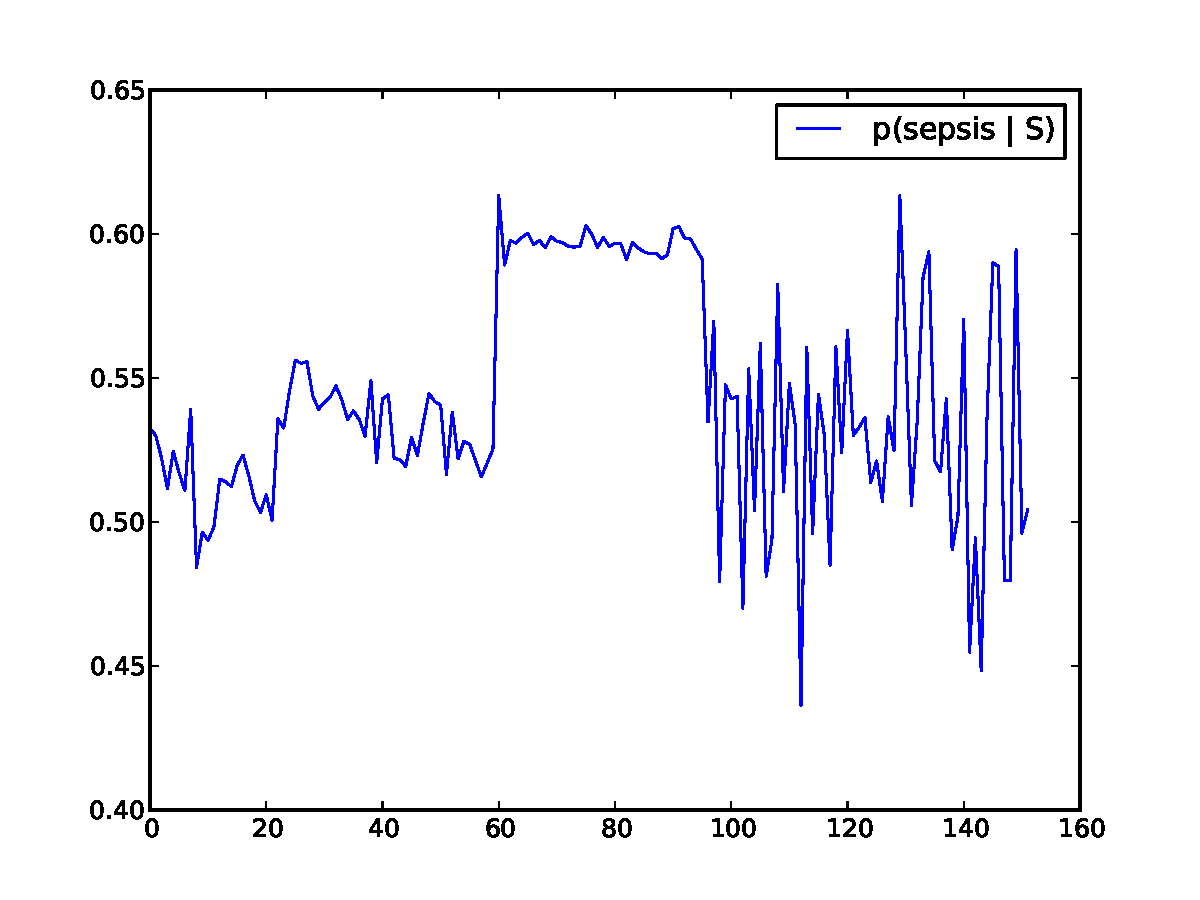
\includegraphics[width=\textwidth]{nn_plots/probs_c0_4}
                \caption{}
                \label{fig:c0_0}
        \end{subfigure}
        \begin{subfigure}[b]{0.4\textwidth}
                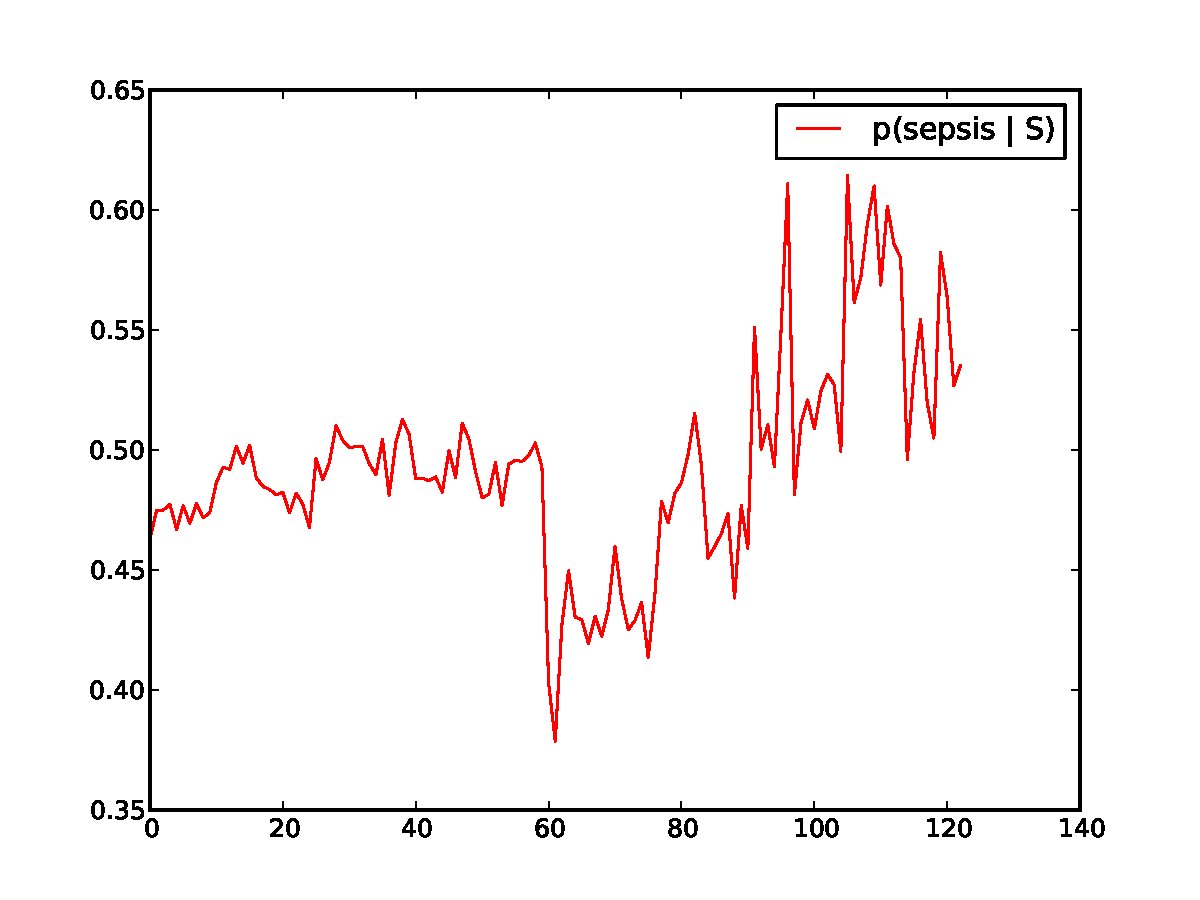
\includegraphics[width=\textwidth]{nn_plots/probs_c1_4}
                \caption{}
                \label{fig:c0_0}
        \end{subfigure}
\caption{Probability of sepsis from beginning to end of individual dev (validation) records. The left column (blue) corresponds to patients who only have SIRS, while the right column (red) corresponds to those who develop either severe sepsis or septic shock by the end of the time series. These results are due to a network with 120 input nodes and 100 hidden layer nodes.}\label{fig:probs}
\end{figure}
The goal of this section is the early prediction of septic shock, rather than just the classification of it in static window. Figure ~\ref{fig:probs}
illustrates preliminary results for this task. In each patient, we slide a window over the time series, and generate $p(sepsis \mid frame)$. Before calculating these probabilities, the network was trained using the techniques discussed in the previous session. Further, results were
only reported for networks which achieved an error rate of .30 or less on the dev set (see ~\ref{fig:dev}). 
\\
\\
Ideally, we would like to see that the $p(sepsis \mid frame_{t})$ increases over time for the patients with severe sepsis and septic shock
and remains relatively constant for patients with SIRS. Additionally, it would be desirable for the $p(sepsis \mid frame_{t})$ to be 
higher in general for those who go on to develop septic shock or severe sepsis than those who develop SIRs. Given our preliminary
data, it is unclear if we can affirm either of these statements.   

\subsection{Discussion}

In \textit{Approach} we describe that the input to the network is a one hour frame of mean heart rate and heart rate standard deviation.
The two features are extracted from 1 minute intervals in the original heart rate. Initially, we attempted to use the raw 2 Hz heart rate directly,
but this suffered from slow training and near chance dev set accuracy. We also extracted these features at intervals of 
15 and 7.5 minutes. Due to such extreme downsampling, the data was much faster to process, but accuracy was no better than chance. Experimentally, we found that features extracted at one minute intervals retained enough structure in the data for learning to occur (see \textit{Preliminary Results}) while being computationally tractable.
 
\subsection{Future Work}

We observed numerical instability and overfitting in networks with several layers. However, we never implemented the sophisticated pretraining
methods characteristic of DNNs. After incorporating these techniques, we will explore what, if any, advantage deep neural networks provide
us in this domain.
\\
\\
Our current framework can accurately classify a one hour frame of heart rate as septic or not septic when the input is unambiguous. However,
when used to predict the future onset of sepsis, results under this system are inconclusive (see \textit{Preliminary Results}).
\\
\\
It is possible that heart rate alone doesn't have enough structure to adequately predict septic shock hours in advance. We will incorporate
additional physiological signals, such as blood pressure and respiratory rate as features to the neural network.

\subsection{Data}

The data for this task consists of heart rate sampled at 2 Hz derived from the MIMIC II Waveform Database. For neural network training, we use a 486 record subset which 
serves as the training, dev, and test sets. 
Each record contains heart rate for an ICU patient with SIRS, severe sepsis or septic shock, with at least
12 hours preceding the event.

\section{Reliable Classification: deriving the optimal decision policy}

\subsection{Introduction}
Since we are interested in applying our system in a clinical setting, we need a way to define a decision policy that makes decisions relative to a clinician's tolerance for false positives and false negatives. To achieve this we derive an optimal decision policy over time that uses an asymmetric cost function to incorporate clinical concerns about the relative cost of different misclassifications. We also introduce the idea of refusing to predict. Instead of forcing the system to always choose a class, we add a state that corresponds to saying ``I don't know". This state provides the clinician with additional information that would not be captured in a traditional classification model. When the model refuses to predict, it is essentially telling the clinician that it needs more information in order to make its decision because it is not sufficiently confident in any one class. In this section we demonstrate how to derive and implement this decision policy over a time sequence and show its application first to synthetic data and then to decision values output from an SVM trained to do septic shock prediction.

\subsection{Related Work}

Adding the notion of rejection (i.e.\  refusing to predict) allows the classifier to avoid misclassification by instead refusing to predict. As stated by Chow \cite{Chow1970} the optimal strategy is one that minimizes the rate of rejection. For a single time point, Chow shows how to formulate the decision policy of when to reject in terms of a rejection threshold. He similarly formulates the error in terms of that same threshold by noting that the expected cost of error is the expected cost of rejecting minus the expectation of being correct. This rejection threshold can then relate the expected cost of rejecting to the expected cost of misclassification and allow the user to trade off between them. 

Grall-Ma\"{e}s and  Beauseroy \cite{GrallMaes2009} extend the optimal decision framework by allowing an observation to be assigned to a subset of the classes. Assigning an observation to the set of all classes corresponds to refusing to predict and assigning an observation to a set with only one class corresponds to predicting that class without ambiguity. Grall-Ma\"{e}s and  Beauseroy derive the optimal decision policy for assigning an observation to a set given a cost matrix and performance constraints. Performance constraints are, for example, the false positives for this class must be below a given threshold or the false positives for a given subset must be below this level.

Santaniello et al.\ \cite{Santaniello2012} formulate a transition detection problem where they learn a decision policy to decide when a change of state has occurred in a time sequence. In particular, they derive a decision policy for quickest detection, where they want to detect the change point as early as possible with sufficient confidence. To encourage early detection, they include the expected distance of the current time from the actual change time in the cost function.

\subsection{General Problem Set Up}

\begin{figure}[ht]
  \begin{center}
    \begin{tabular}{cc}
      % model_reclas

\begin{tikzpicture}

% define nodes

% decisions

\node[latent,minimum size=9mm] (up) {$u_{t-1}$};
\node[const, left=2cm of up,minimum size=9mm] (ud) {$\ldots$};
\node[latent, right=3cm of up,minimum size=9mm] (ut) {$u_{t}$};
\node[latent, right=3cm of ut,minimum size=9mm] (un) {$u_{t+1}$};
\node[const, right=2cm of un,minimum size=9mm] (uf) {$\ldots$};
% truth
\node[const, above=2cmof up,xshift=-3cm,minimum size=9mm] (yd) {$\ldots$};
\node[latent, above=2cm  of up,minimum size=9mm] (yp) {$y_{t-1}$};
\node[latent, right=3cm  of yp, minimum size=9mm] (yt) {$y_{t}$};
\node[latent, right=3cm  of yt,minimum size=9mm] (yn) {$y_{t+1}$};
% prediction
\node[latent, above=of yp, xshift=-1cm,minimum size=9mm] (yhp) {$\hat{y}_{t-1}$};
\node[latent, above=of yt, xshift=-1cm,minimum size=9mm] (yht) {$\hat{y}_{t  }$};
\node[latent, above=of yn, xshift=-1cm,minimum size=9mm] (yhn) {$\hat{y}_{t+1}$};
\node[const, right=3cm  of yhn,minimum size=9mm] (yf) {$\ldots$};
% observation
\node[obs, above=of yhp,minimum size=9mm] (xp) {$x_{t-1}$};
\node[obs, above=of yht,minimum size=9mm] (xt) {$x_{t}$};
\node[obs, above=of yhn,minimum size=9mm] (xn) {$x_{t+1}$};
% intervention
\node[obs, right=1cm of xp,minimum size=9mm] (rp) {$r_{t-1}$};
\node[obs, right=1cm of xt,minimum size=9mm] (rt) {$r_{t}$};
\node[obs, right=1cm of xn,minimum size=9mm] (rn) {$r_{t+1}$};


% edges

\edge {xp,yd} {yhp};
\edge {xt,yp} {yht};
\edge {xn,yt} {yhn};

\edge{rp, yhp} {yp};
\edge{rt, yht} {yt};
\edge{rn, yhn} {yn};
\edge {yn} {yf};
\edge {yp, ud} {up};
\edge {yt, up} {ut};
\edge {yn, ut} {un};
\edge {un} {uf};

% plates

\plate {} {(yp)(yt)(yn)(up)(ut)(un)}{};

\end{tikzpicture}
    \end{tabular}
  \end{center}
  \caption{Reliable Classifier model as a Bayesian network}
\label{fig:reclas_bnet}
\end{figure}


\begin{align*}
X &= x_0, x_1, \ldots, x_T \text{ sequence of observations}\\
R &= r_0, r_1 \ldots, r_T \text{ sequence of clinical interventions}\\
\hat{Y} &= \yh_0, \yh_1, \ldots, \yh_T \text{ sequence of predicted class labels, $\yh_i \in \{1,\ldots, C\}$}\\
Y&=y_0,y_1,\ldots,y_T \text{ sequence of true labels, $y_i \in \{1,\ldots, C\}$}\\
U&=u_0,u_1,\ldots,u_T \text{ a decision policy, $u_i \in \{1,\ldots, C, C+1\}$}\\
S &\in \R^{C+1 \times C \times T}, S_{i,j}^{(t)} \text{ is the cost of choosing label $i$ instead of label $j$ at time $t$}\\
\bar{C} &= \{1,\ldots, C\} \text{ set of possible classes}\\
\hat{C} &= \{1,\ldots, C,C+1\} \text{ set of possible decisions}
\end{align*}

At each time $t$ the system either chooses the class $c \in \{1,\ldots, C\}$ that minimizes the expected loss over the time sequence $0\ldots T$ or it refuses to make a decision, corresponding to choosing $c = C+1$. Each $\yh_t$ is a probability distribution over possible the possible classes $\bar{C}$. If there is a clinical intervention $r_t$ at the current time $t$, e.g.\ a doctor prescribes pressors or performs some other action that provides a diagnosis, we define $P(y_t=j)$ to be $P(y_t=j|r_t)$. However, since we are performing a continuous monitoring task, the majority of time points will not have a clinical intervention associated with it. In these cases we use the distribution from the classifier $\yh_t$ and define $P(y_t=j)$ to be $P(\yh_t=j|x_t, y_{t-1})$. We then feed the distribution $y_t$ to our classifier so that the predicted distribution over classes $\yh_{t+1}$ incorporates knowledge about clinical interventions into the classification process. Instead of defining the distribution $y_t$ as either $r_t$ or $\yh_t$, we could instead define it as a mixture of the two distributions based on our confidence in the classifier's predictions. 

The decision $u_t$ is influenced by the distribution over all possible class labels $y_t$ and the previous decision $u_{t-1}$. The motivation for allowing the previous decision to influence the current decision is two-fold. First this can act as a smoothing function and capture the intuition that patients show a gradual transition from one disease state to the next, and prevents situations like repeatedly alternating between two disease states instead of staying in one state until the classifier is sufficiently confident to advance to a new disease state. The second benefit of this dependency between successive decisions is that it allows us to prevent overly long rejection periods, where the classifier continuously refuses to predict. We can do this by progressively down-weighting the probability of rejection given the history of rejection.

\subsection{Expected Loss}
Define the expected posterior loss at time $t$ of making decision $u_t=i$ given that the true label is $y_t=j$ and the previous decision was $u_{t-1}=h$ as follows:

\begin{align}
\E[L(u_t|y_t, u_{t-1})] &= \min_{u_t} \Big\{ \sum_{i \in \hat{C}} \sum_{j \in \bar{C}} S_{i,j}^{(t)} P(y_t=j)P(u_t=i|u_{t-1})\I(u_t=i)\Big\}\\
&= \min_{u_t \in \hat{C}} \Big\{ \sum_{j \in \bar{C}} S_{u_t,j}^{(t)} P(y_t=j)P(u_t|u_{t-1})\Big\}
\label{eqn:exploss}
\end{align}

The cost matrix $S$ gives the user a way of making tradeoffs between false positives and false negatives and between refusing to predict and having less confidence in the predictions. Critically, we allow for an asymmetric cost function and we do not assume that the cost function is non-decreasing over time. Allowing for an asymmetric cost function enables the clinician to introduce class specific penalties for misclassification and for refusing to predict. This captures the belief that, in a clinical setting, not all mistakes are of the same importance. For instance, predicting that a patient is normal, when in fact they are in septic shock is a more serious mistake than predicting that a patient is normal when they actually meet the SIRS criteria. 

A possible extension to the loss function is to add the entropy of the current probability distribution to the cost of predicting a given class or to subtract it from the cost of refusal. This would help prevent situations where a couple of classes share almost all of the probability mass, but are both equally costly, and thus it is unclear which the system should actually predict. Adding the entropy term would make it more expensive to make any prediction when there is high entropy in the probability distribution.

\subsection{Deriving the Optimal Decision}

Our goal is to learn a decision policy that makes the decision $u_T$ that minimizes the expected loss over the observations and interventions over time $0\ldots T$. We introduce a discount factor $\beta \in [0,1]$ to assign less weight to the expected loss of decisions made far in the past. For $\beta = 0$, we discount all but the expected loss of the most recent decision. For $\beta = 1$, we give the expected loss of all decisions equal weight.

% Bellman equations to learn optimal decision

Let $V(y_T)$ be the value of the expected posterior loss minimized by a decision policy $\{u_t\}_{t=0}^{T}$. At time $T$ we make the decision $u_T$ that is the argmin of (\ref{eqn:bellman}).

\begin{align}
V(y_T) &= \min_{\{u_t\}_{t=0}^{T}} \Big\{ \sum_{t=0}^T \beta^{T-t}\E[L(u_t|y_t, u_{t-1})] \Big\}\\
&= \min_{u_T \in \hat{C}} \Big\{  \beta^{0}\E[L(u_T|y_T, u_{T-1})] + \min_{\{u_t\}_{t=0}^{T-1}} \beta \sum_{t=0}^{T-1} \beta^{T-1-t}\E[L(u_t|y_t, u_{t-1})] \Big\}\\
&= \min_{u_T \in \hat{C}} \Big\{  \E[L(u_T|y_T, u_{T-1})] + \beta V(y_{T-1})\Big\} \label{eqn:bellman}
\end{align}

From this we see that the system will either make the decision $u_T = c \in \bar{C}$ that minimizes the expected loss over the sequence or it will refuse to predict, equivalent to choosing $u_T = C+1$. Let $c = \argmin_{c\in \bar{C}} \big\{ \E[L(C+1|y_T, u_{T-1})] + \beta V(y_{T-1})\big\}$.

\begin{equation}
u_T = 
\begin{cases}
C+1 &  \text{if } \E[L(C+1|y_T, u_{T-1})] + \beta V(y_{T-1}) <   \E[L(c|y_T, u_{T-1})] + \beta V(y_{T-1})\\
c \in \bar{C} & \text{otherwise}
\end{cases}
\end{equation}

Since $ \beta V(y_{T-1})$ is the same value in both cases, this condition reduces to choosing $C+1$ if  $\E[L(C+1|y_T, u_{T-1})] <   \E[L(c|y_T, u_{T-1})] $ or equivalently, assuming $ \E[L(c|y_T, u_{T-1})]  > 0$, i.e.\ that $S^{(T)}_{c,j} \geq \forall j \in \bar{C}$ and that $ S^{(T)}_{c,j}  >0 $ for some $j \in \bar{C}$,

\begin{equation}
u_T = 
\begin{cases}
C+1 &  \text{if } \frac{\E[L(C+1|y_T, u_{T-1})]}{\E[L(c|y_T, u_{T-1})]} < 1\\
c \in \bar{C} & \text{otherwise}
\end{cases}
\end{equation}


\subsection{Dynamic Programming}

% Implementing dynamic programming to solve Bellman equations
Define a matrix $V \in \R^{C+1\times T}$ where each entry is defined as
\begin{align}
V_{i,t} &=  \E[L(u_t=i|y_t, u_{t-1}=\argmin_{k} V_{k,t-1})] + \beta \min_{k\in\hat{C}} V_{k,t-1}\\
&= \sum_{j \in \bar{C}} S_{i,j}^{(t)} P(y_t=j)P(i|u_{t-1}=\argmin_{k\in\hat{C}} V_{k,t-1}) + \beta \min_k V_{k,t-1}
 \label{eqn:dp_step}
\end{align}

% initialize the model at time 0
At time $t=0$, we do not have any history of observations or decisions, so we initialize our decision process with $V_{i,0}$ as the expected loss of making decision $i$
\begin{align}
V_{i,0} &=  \E[L(u_0=i|y_0, \emptyset)] \\
%&= \sum_{i \in \hat{C}} \sum_{j \in \bar{C}} S_{i,j}^{(0)} P(y_0=j)P(u_0=i)\I(u_0=i) \\
&=  \sum_{j \in \bar{C}} S_{i,j}^{(0)} P(y_0=j)P(u_0=i)\label{eqn:dp_init}
\end{align}


In order to find the optimal decision at time $T$, we initialize our model at time $t=0$ as shown in (\ref{eqn:dp_init})and then for each possible class $i$, we compute the value of $V_{i,t+1}$ at the next time step as shown in (\ref{eqn:dp_step}). We iteratively continue the process until we reach the current time point $t=T$. We then make decision $u_T = \argmin_{i \in \hat{C}} V_{i, T}$, which is the decision at time $T$ that minimizes the expected loss over the observed period. For the purpose of computational efficiency, we only need to maintain the previous column $V_{1\ldots C+1, t-1}$ in order to calculate the values of $V_{1\ldots C+1, t}$ at the current time point. If we want to learn a decision policy over the entire time sequence, we simply maintain a vector $U = [u_0, \ldots, u_T]$, where $u_t =  \argmin_{i \in \hat{C}} V_{i, t}$.

At each time step we perform $(C+1)(4C)$ operations, so the total complexity is $O(TC^2)$. Assuming that we remember the values computed at the previous time step, the update for each new observation is $O(C^2)$.


The preceding update assumes that we cannot retroactively update our decisions even if doing so might allow us to make a lower-cost decision at the current time. If we instead allow our system to reinterpret past decisions in order to minimize the expected loss at the current time, the initialization of the dynamic programming algorithm remains the same, but the update is instead minimized over all possible previous decisions (\ref{eqn:dp_step2}). The complexity for each new observation then becomes $O(TC^3)$, because each new observation now requires $(C+1)(C+1)(4C)$ operations. Moreover, we need to maintain a matrix of the decisions $u_{t-1}$ that minimized the expected loss at the next time step. Once we reach the current time $T$ we can backtrack through this matrix to see the sequence of decisions that led to the optimal decision at time $T$. 

\begin{align}
V_{i,t} &= \min_{u_{t-1} \in \hat{C}} \big\{ \E[L(u_t=i|y_t, u_{t-1})] + \beta V_{u_{t-1},t-1}\big\}\\
&=  \min_{u_{t-1} \in \hat{C}} \big\{  \sum_{j \in \bar{C}} S_{i,j}^{(t)} P(y_t=j)P(i|u_{t-1}) + \beta V_{u_{t-1},t-1}\big\}
 \label{eqn:dp_step2}
\end{align}




\subsection{CRF Derivation}

The input to the reliable classifier is a sequence of distributions over predicted class labels $Y = y_0, y_1, \ldots, y_T$, where each $y_t$ is a probability distribution over the possible classes $\{1,\ldots,C\}$ given the previous distribution $y_{t-1}$ and the observations up to time $t$. We explore a CRF framework for learning this predicted distribution at each time step.

At each node $y_t$ we have the node potential $P(y_t|X)$ and the edge potential $P(y_t, y_{t-1})$. We assume that the univariate potential $P(y_t|X)$ is given from the output of an SVM or other classifier. We can then take these univariate potentials and chain them into a CRF in order to incorporate information about temporal dynamics. For all pairs of classes $i,j \in \{1,\ldots,C\}$ we define a feature function $f_{i,j} = \mathbb{1}(y_{t-1}=i, y_{t}=j)$ and learn a corresponding weight $\lambda_{i,j}$. Here we have defined $\lambda_{i,j} = P(y_{t-1} = i,y_t=j)$ for $t >1$ and $\lambda_{i,j} = P(y_t=j)$ for $t =1$.

We then use the forward algorithm to compute the probability the probability of a class label $j$ given the observations up to the current time $t$ and the sequence of previous label distributions, $P(y_t =j| Y_{1:t-1}, X_{1:t}) $ for each $j \in \bar{C}$. We start by initializing $\alpha_{1,j} = P(y_1=j)P(y_1=j|x_1)$. We then compute $\alpha_{2:T}$ by recursively computing $\alpha_{t,j} = \sum_{i \in \bar{C}}\alpha_{t-1,i}P(y_t=j|X_{1:t})P(y_{t-1} = i,y_t=j)$. For $t=1,\ldots, T$, we compute $P(y_t =j| Y_{1:t-1}, X_{1:t}) $ as in (\ref{eqn:crf_inference}).

\begin{equation}
P(y_t=j | Y_{1:t-1}, X_{1:t}) = \frac{\alpha_{t,j}}{\sum_{j \in \bar{C}}\alpha_{t,j}} \label{eqn:crf_inference}
\end{equation}
 
Once we have $\alpha_{t,j} $, if we add a new observation $x_{t+1}$, we can easily compute $P(y_{t+1}=j | Y_{1:t}, X_{1:t+1})$ using (\ref{eqn:crf_inference}).

\subsection{Simulation with synthetic data}

In order to test the reliable classification, we define four classes, where the data from each class is sampled from a Gaussian with means 0,3,6,8 and variances 3,3,2,1 respectively. Each sample is 250 time steps long and there are 1000 samples. At each time step the sample is drawn from one of the four classes and the sample transitions between classes based on a given transition matrix and initial probabilities.


We use Kevin We use a 2DBN implemented with Kevin Murphy's BayesNet Toolbox for Matlab to calculate the marginal probabilities. Since we focus on learning the decision policy rather than the probability estimation task, we provide the 2DBN with the transition matrix, class-specific Gaussians, and initial probabilities used to generate the data.

We also calculate the distributions over classes conditioned on the observations using the above CRF derivation. Since we know the four distributions that the data is drawn from, we define four feature functions $f_j(y) = \one(y=j)$ for $j \in \bar{C}$ with respective weights $\lambda_j = P(x | \mu_j, \Sigma_j)$ with a normal PDF.  We also have feature functions for each possible pair of classes $i,j \in \bar{C}$ where  $f_{i,j} = \one(y_{t-1}=i,y_t=j)$ and $\lambda_{i,j} = Ti,j$, the value from the transition matrix. For the simulation we do not address the situation where we have a doctor intervention (i.e.\ $R=\emptyset$). 

We will consider how different parameterizations of the cost matrix allow us to trade off between the cost of misclassification and the cost of refusing to predict. We will also investigate how to set the cost matrix to encourage early detection.

If we have a decision policy without a notion of refusing to predict, then ideal behavior of our decision policy with rejection is to refuse to predict whenever the previous decision policy made an incorrect classification and to predict the same class whenever it made a correct prediction. In order to evaluate different settings of the cost matrix and other parameters, we compare the fraction of mistakes that are rejection in the decision policy with rejection and the fraction of correct classifications that are correctly classified. Since we use the same policy for choosing the best cost class among the classes for both the decision policy with and without rejection, there will not be mistakes that become correct answers in the new model and there will not be correct answers that become incorrect. The poster (slide 22) compares the decision policy for different costs of class substitution and refusing to predict and demonstrates how the decision policy can make different tradeoffs between tolerances for false positives, false negatives, and refusing to predict.

\subsection{Septic Shock Early Detection}

% TASK DESCRIPTION
We apply our method to the task of early prediction of septic shock. We are given the output from an SVM that predicts whether or not a person has septic shock and has a corresponding label: not septic shock, yes septic shock, and uncertain \cite{Paxton2013}. A patient is labeled as having septic shock based on when a doctor records it in the EMR. However, this provides a noisy label since it does not denote the true onset of septic shock, but rather when a doctor treated the patient for septic shock. Moreover, developing septic shock is a gradual process and is challenging to identify the precise moment of septic shock onset. In order to account for this, the twelve hours preceding the documented septic shock onset are labeled as uncertain. A patient may also be labeled as uncertain if there are confounding factors that prevent us from knowing whether or not they developed septic shock. For instance, the caregiver may decide to proactively administer antibiotics before confirming that a patient has fully developed septic shock. If the patient does not subsequently develop septic shock, then it is unknown whether the patient never would have developed septic shock or whether they were going into septic shock, but the medical intervention stopped the progression to septic shock. 

We use a sigmoid function $S(x) = \frac{1}{1+e^-x}$ to map the values output from the SVM to the range $[0,1]$ and interpret this as a univariate potential that a patient has septic shock at that time. Let $\pi_t$ represent the univariate potential at time $t$.

Let $H$ denote healthy/not septic shock and let $K$ denote septic shock. There are four possible class sequences $(y_{t-1},y_t)$ that occur in the dataset: $(H,H), (H,K), (K,H), (K,K)$. We define the probability $P(y_{t-1}=H, y_t=K)$ as the fraction of patients who develop septic shock and $P(y_{t-1}=H, y_t=H) = 1 - P(y_{t-1}=H, y_t=K)$. In the dataset we never observe a patient transition from septic shock to not septic shock. Currently we have $P(y_{t-1}=K, y_t=K) = 1$ and  $P(y_{t-1}=K, y_t=H) = 0$, which leads to a transition matrix $T = \begin{bmatrix}0.995&0.005\\0&1\end{bmatrix}$

In the poster slides, we show four examples of the the decision policy model applied to the decision values output by the SVM. For each example we show the observations progressing in time from left to right. From top to bottom there is the decision value output by the SVM mapped to $[0,1]$, the marginal probability of each class given the observations up until that time point inferred from the CRF, the true labels of the data, and the labels that the decisions made by the decision policy. All of these examples were generated using 0/1 loss for misclassification and a uniform 0.3 cost of refusing to predict.

As can be seen in all of the examples, the CRF substantially smooths out the probabilities of each class. The probability of the more likely class quickly approaches 1. This is most likely caused by the transition matrix, which makes it very unlikely to change between classes. As a result, seeing a few samples in a row with significant probability of one of the classes causes it to put extremely high probability on the sample belonging to that class.

In example one (slide 25), we see that not septic shock starts out as the most likely class, but around sample 30 the decision values output by the SVM rank septic shock as the more likely state. However, because the CRF incorporates temporal information, it smooths away the increased probability of septic shock and the decision policy continues to correctly select not septic shock. We could adjust the systems sensitivity by increasing its tolerance for false alarms on septic shock, which corresponds to decreasing the cost of predicting septic shock when the true label is not septic shock. Alternatively, we could lower the cost of refusing to predict, which would allow us to maintain the same false alarm rate, but still alert the clinicians that the patient may be entering septic shock or that additional evaluation is needed.

In example two we see another example where the CRF smooths out the class probabilities and removes some of the uncertainty from the raw decision values by incorporating temporal information.

In example three, there is an example of a patient who is in septic shock; however the decision values output by the SVM still initially rank not septic shock as the more likely class. The high initial probability on not septic shock and low probability of transitioning from not septic shock to septic shock cause the CRF to put high weight on not septic shock, which causes the system to initially misclassify it as not septic shock. Later, the probability of septic shock increases and the decision policy starts choosing septic shock after a short period of refusing to predict. Again, the precise behavior of the decision policy could be tweaked to allow for more or less false positives and false negatives and to also adjust the frequency of not predicting.

Example four shows an instance where the true label of the patient was unknown. This could be caused by several scenarios such as the patient being preemptively prescribed antibiotics, thus masking whether or not they would have developed septic shock. Although the true label is uncertain, the SVM and CRF rank septic shock as the more likely state. The decision policy initially predicts not septic shock and then refuses to predict, probably due to the overly high initial probability of not septic shock, but then predicts septic shock, until it later sees an increase in the probability of not septic shock.

\subsection{Discussion and Future Work}

One of the problems with the CRF probabilities is that it does not have a global notion of how long the patient has been in a given state. Instead of modeling how likely we are to stay in septic shock for a given amount of time, we simply model how likely are we to transition from septic shock to septic shock. Modifying the model from a CRF to a semi-Markov CRF would allows us to model the duration of each state. Incorporating information about the likely duration of septic shock could help prevent situations where a patient switches between septic shock and not septic shock. Moreover it would allow us to incorporate clinical knowledge about how long it takes from the first observation of SIRS to transition into septic shock or from severe sepsis to septic shock once we transition to modeling the four classes instead of a binary classification task.

Additionally, the transition matrix and other parameters in the CRF and cost function are currently hand-defined and tweaked. In future work we would like to learn these parameters from the data. This could also help correct the model's tendency to over estimate the probability of the current class.

\section{Overall Discussion and Future Work}

In this project we used heart rate exclusively to distinguish between sepsis states. However, results from the HMM tagger demonstrate
that while it is possible to distinguish between SIRS and the septic shock, it is difficult to distinguish between the different types
of sepsis (e.g., severe sepsis and septic shock). Physiological data has predictive power, but additional representations and possibly additional signals may be beneficial. For instance, early predictive ability of the neural network may be applified by augmenting  heart rate with respiratory rate and blood pressure.
\\
\\
Integration of the three components of this project is an important, but currently unmet goal of this project. Ideally, each component of
this project will interact with each other in a pipeline. For instance, the HMM tag sequence can be interpreted as categorical features and 
input to the neural network. Alternatively, the probability of observation sequence under each HMM model can be directly used as input into
the decision policy system. The output of the neural network are conditional probabilities which can serve as input into the decision policy 
system.

\bibliographystyle{plain}

\bibliography{PhysMod,dnn,ref}

\end{document}
